\documentclass{article}
\usepackage{amsmath}
\usepackage{amssymb}
\usepackage{graphicx}
\usepackage{hyperref}
\usepackage[version=4]{mhchem}

\title{Example 5}
\date{}

\begin{document}
\maketitle

The radii are 10 feet and 17 feet of two intersecting circles. The value for the distance between the centers of the circles is 12 . Find the length of the common chord.\\
(A) \(3 \sqrt{11}\)\\
(B) \(\frac{65}{6}\)\\
(C) \(4 \sqrt{6}\)\\
(D) 10

Solution: (D).\\
Let the centers be \(O\) and \(O_{1}\) of two circles. The intersecting\\
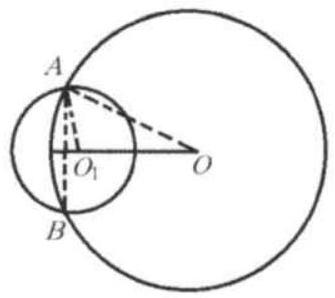
\includegraphics[width=\textwidth]{images/178.jpg} point are \(A\) and \(B\). Connect \(O A, A B, O_{1} A\).\\
In \(\triangle O O_{1} A, O A=13, O O_{1}=12, O_{1} A=5\).\\
Since \(5^{2}+12^{2}=13^{2}\), we know that \(\angle A O_{1} O=90^{\circ}\).\\
So the common chord \(A B\) goes through \(O_{1}\).\\
Thus \(A B=10\).


\end{document}
